\documentclass{uc3mpracticas}

\usepackage{helvet}
\usepackage{caption}
\renewcommand{\familydefault}{\sfdefault}


%%%%%%%%%%%%%%%%%%%%%%%%%%%%%%%%%%%%%%%%%%%%%%%%%%%%%%%%%%%%%%%%%%%%%%%%%%%%%%%%
%%%                   Plantilla Prácticas UC3M                               %%%
%%%                Universidad Carlos III de Madrid                          %%%
%%%                   Alejandro Valverde Mahou                               %%%
%%%%%%%%%%%%%%%%%%%%%%%%%%%%%%%%%%%%%%%%%%%%%%%%%%%%%%%%%%%%%%%%%%%%%%%%%%%%%%%%

%Permitir cabeceras y pie de páginas personalizados
\pagestyle{fancy}

%Path por defecto de las imágenes
\graphicspath{ {./images/} }

%Declarar formato de encabezado y pie de página de las páginas del documento
\fancypagestyle{doc}{
  %Cabecera
  \headerpr[1]{Sistemas de Producción}{}{Ingeniería del Conocimiento}
  %Pie de Página
  \footerpr{}{\textbf{UC3M}}{{\thepage} de \pageref{LastPage}}
}

%Declarar formato de encabezado y pie del título e indice
\fancypagestyle{titu}{%
  %Cabecera
  \headerpr{}{}{}
  %Pie de Página
  \footerpr{}{}{}
}


\appto\frontmatter{\pagestyle{titu}}
\appto\mainmatter{\pagestyle{doc}}


\begin{document}
  %Comienzo formato título
  \frontmatter


  %Portada 1 (Centrado todo)
  \centeredtitle{Images/LogoUC3M.png}{Grado en Ingeniería Informática}{Curso 2020/2021}{Ingeniería del Conocimiento}{Práctica 1: Sistemas de Producción}

  \vspace{55mm}

  \authors{Alba Reinders Sánchez}{100383444}{Alejandro Valverde Mahou}{100383383}{}{}{Grupo 83}{Leganés}

  \newpage

  %Índice
  \tableofcontents

  \newpage

  %Comienzo formato documento general
  \mainmatter

  \section{Introducción}

En esta primera práctica se aborda la implementación de un \textbf{sistema de producción} (\textit{SP}) en CLIPS que lleve a cabo la ejecución de una sesión de un especialista con un paciente en la que interactúan un humano y un robot \textit{NAO}, donde este último adopta el papel de especialista.

\begin{figure}[!h]
  \centering
  \includegraphics[width=.25\linewidth]{Images/nao.png}
  \caption*{Robot \textit{NAO}}
\end{figure}


En concreto, se crea un \textit{SP} con toda la información respecto a los personajes y el entorno en el que se lleva a cabo la interacción, así como posibles desviaciones durante la sesión en las que el robot debe reaccionar y modificar sus acciones en consecuencia.

\vspace{2mm}

La interacción entre el paciente y el robot se realiza a través del desarrollo de 2 juegos: el \textbf{Twister} y el \textbf{Tres en raya}. Además, el sistema está adecuado para tratar con pacientes que puedan presentar 2 personalidades distintas, aparte del comportamiento base, \textbf{despistado} y \textbf{enérgico}.

\vspace{2mm}

Se han elegido estos juegos por ser ejemplos de actividades sencillas, que requieren de un número reducido de reglas, para demostrar las aplicaciones de los \textit{SP}. Por el mismo motivo, se han elegido únicamente 2 posibles comportamientos básicos. Si se deseara aplicar sobre un problema real no serían suficientes, y sería necesario tener en cuenta un mayor número de personalidades.


\begin{figure}[!h]
  \centering
  \begin{minipage}{.52\textwidth}
    \centering
    
\includegraphics[width=.5\linewidth]{Images/3enraya.png}
    \caption*{Juego del Tres en Raya}
  \end{minipage}%
  \begin{minipage}{.52\textwidth}
    \centering
    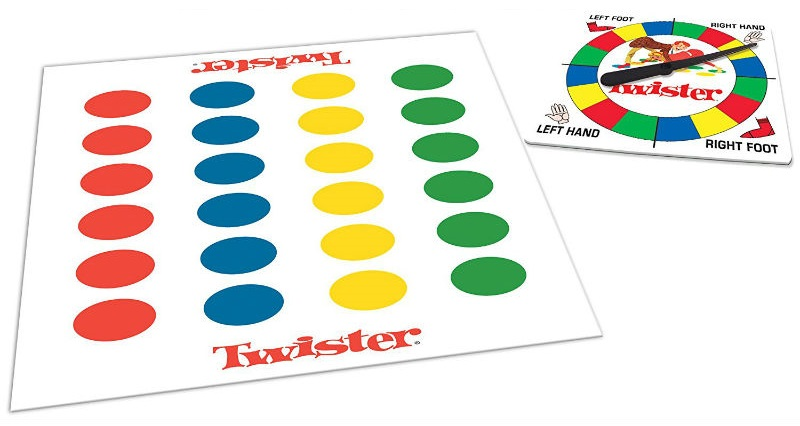
\includegraphics[width=.8\linewidth]{Images/twister.jpg}
    \caption*{Juego del Twister}
  \end{minipage}
\end{figure}

El documento consiste en el manual técnico con la descripción de la implementación, el manual de usuario con la explicación de cómo usar el programa, las pruebas realizadas y el análisis de los resultados, y para finalizar una serie de conclusiones y comentarios personales.


  \newpage

  \section{Manual técnico}

  El \textit{SP} está compuesto por la \textbf{ontología} y las \textbf{reglas}. A continuación, se explican ambas justificando todas las decisiones que se han tomado durante la implementación.

  \vspace{2mm}

  Los flujos de acciones que se han planteado para resolver los problemas son los siguientes, donde los estados de color rojo solo se pueden realizar si el \textit{paciente} es \textit{enérgico} y los de color verde si el \textit{paciente} es \textit{despistado}.

  \begin{figure}[!h]
    \centering
    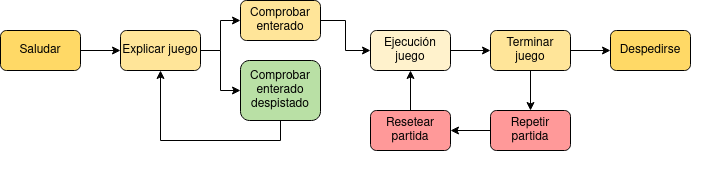
\includegraphics[width=.75\linewidth]{Images/flujo_sesion1.png}
    \caption*{Flujo genérico de una sesión}
  \end{figure}

  \begin{figure}[!h]
    \centering
    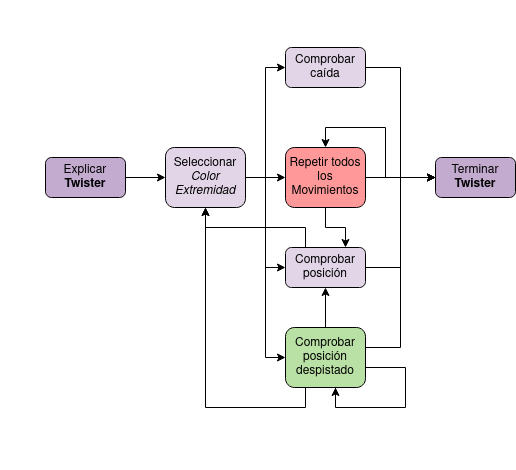
\includegraphics[width=.75\linewidth]{Images/flujo_sesion2.png}
    \caption*{Flujo del Twister}
  \end{figure}

  \begin{figure}[!h]
    \centering
    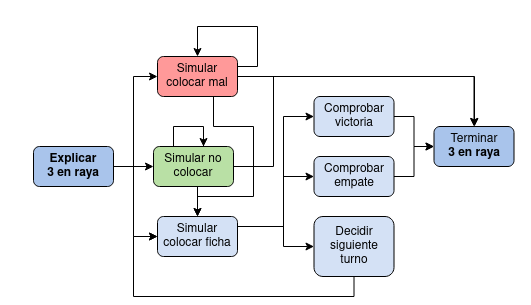
\includegraphics[width=.75\linewidth]{Images/flujo_sesion3.png}
    \caption*{Flujo del Tres en Raya}
  \end{figure}

  \newpage

  \subsection{Ontología}

  La ontología que se plantea para la solución está compuesta de las siguientes clases.

  \begin{itemize}
    \item \textbf{JUEGO} $\rightarrow$ Representa el juego que se va a llevar a cabo a lo largo de la sesión. Contiene, además del nombre (\textit{id}) del juego, la explicación del mismo, junto con la indicación de quién debe empezar (\textit{paciente} o \textit{robot}). Esto se ha decidido porque para cada juego comienza uno de los dos:

    \vspace{1mm}

    En el caso del \textbf{\textit{Twister}}, el \textit{robot} será siempre el que empiece la partida, dado que será el \textit{paciente} el que siempre 'juegue', mientras que el \textit{robot} elige las acciones.

    \vspace{2mm}

    Por otro lado, se ha decidido que para el caso del \textit{\textbf{Tres en Raya}} siempre empiece el paciente. Esto se ha hecho porque, en este juego, el jugador que comienza tiene ventaja y, dado que el juego forma parte de una terapia, se quiere potenciar que el \textit{paciente} gane con mayor probabilidad.

    \item \textbf{CONTROL} $\rightarrow$ Esta clase tendrá una única instancia, y se usa para localizar las distintas operaciones que controlan el sistema en una sola instancia. En el caso excepcional de que se repita la partida (comportamiento que solo puede darse con \textit{pacientes} de personalidad \textit{enérgica}) esta instancia se borra y se reinicia.

    \vspace{2mm}

    Esta clase permite controlar de quién es el turno, el número de ciclos, junto al número máximo de ciclos, el número de fallos, el juego que se lleva a cabo en la sesión, y el número de veces que se repite la partida.

    \item \textbf{PACIENTE} $\rightarrow$ Representa al paciente que está en la sesión. Se ha decidido usar una clase en lugar de un \textit{fact} para representarlo porque, además de la peronalidad del paciente, también almacena el nombre del mismo. Esto se hace para poder enviar mensajes personalizados, y que el paciente se encuentre en un ambienta más cómodo e informal.
    \item \textbf{COLOR} $\rightarrow$ Representa cada uno de los cuatro colores posibles para el juego del \textbf{\textit{Twister}}. Puede ser \textit{rojo}, \textit{verde}, \textit{amarillo} o \textit{azul}.

    \item \textbf{EXTREMIDAD} $\rightarrow$ Representa cada una de las cuatro extremidades posibles para el juego del \textbf{\textit{Twister}}. Puede ser \textit{pie derecho}, \textit{pie izquierdo}, \textit{mano derecha} o \textit{mano izquierda}.

    \item \textbf{ELECCION} $\rightarrow$ Representa cada una de las elecciones o comandos que hace el \textit{robot} y que tiene que realizar el \textit{paciente} en el juego del \textbf{\textit{Twister}}. Además del color y la extremidad elegidas, para poder realizar comprobaciones adicionales, se incluye el número de veces que se ha tenido que repetir una misma elección, y el orden por el que se han dicho.

    \item \textbf{CASILLA} $\rightarrow$ Representa cada una de las 9 casillas del juego del \textit{\textbf{Tres en Raya}}. Además de sus coordenadas, se tiene su valor, que puede ser \textit{vacío} si no se ha colocado nada todavía, o \textit{paciente} o \textit{robot}, en función de quién coloque la ficha.
  \end{itemize}



  \subsection{Reglas}

  \subsubsection{Reglas genéricas}

  Estas reglas son las que sirven para ambos juegos y donde da igual la personalidad del paciente:

  \begin{itemize}
    \item \textbf{\textit{Saludar}}: el \textit{robot} saluda de manera personalizada al \textit{paciente} por su nombre.
    \item \textbf{\textit{Explicar}}: el \textit{robot} explica al \textit{paciente} el juego que se haya elegido.
    \item \textbf{\textit{Comprobar-enterado}}: el \textit{robot} comprueba que el \textit{paciente} se haya enterado de la explicación del juego.
    \item \textbf{\textit{Despedirse}}: el \textit{robot} se despide de manera personalizada del \textit{paciente} por su nombre.
  \end{itemize}

  Si el \textit{paciente} tiene de personalidad \textit{despistado}, existe la regla \textbf{\textit{Comprobar-enterado-despistado}} para repetir la explicación del juego y la regla \textbf{\textit{Demasiadas-equivocaciones-despistado}} para terminar la sesión porque se ha equivocado más de 5 veces y por tanto se considera que el \textit{paciente} puede no estar muy atento para continuar con el juego.

  \vspace{3mm}

  Se añade la regla \textbf{\textit{Repetir-partida}} para volver a jugar otra partida. Esto sucede exclusivamente si el \textit{paciente} es \textit{enérgico}, ya que se considera que puede que tenga más energías para seguir jugando.

  \vspace{1mm}

  Por lo tanto, una vez que se acaba una partida se activa esta regla y, dependiendo del juego, las siguientes: \textbf{\textit{Resetear-partida-tres-en-raya}} y \textbf{\textit{Resetear-partida-twister}}. Estas sirven para reiniciar las variables del juego.

  \vspace{2mm}

  Además, se crea la regla \textbf{\textit{Auxiliar-fin-reseteo}}, que lo que hace es finalizar el proceso de reinicio de variables.

  \vspace{2mm}

  Por último, se tiene la regla \textbf{\textit{Demasiadas-equivocaciones-energico}}, la cual tiene como fin terminar la sesión si el \textit{paciente} intenta colocar un ficha cuando no es su turno más de 3 veces. Este comportamiento es exclusivo del \textit{enérgico}, ya que se considera que ha hecho demasiadas trampas para una sola partida.




  \subsubsection{Reglas Twister}

  En cuanto a las reglas exclusivas para el \textit{\textbf{Twister}}, para un comportamiento normal, se crean las siguientes:

  \begin{itemize}
    \item \textbf{\textit{Robot-selecciona}}: el \textit{robot} selecciona de forma aletoria un color y una extremidad para que el \textit{paciente} realice la acción.
    \item \textbf{\textit{Comprobar-posicion}}: el \textit{robot} comprueba que el \textit{paciente} ha realizado correctamente la acción que le ha dicho y aumenta el contador de ciclos.
    \item \textbf{\textit{Comprobar-caida}}: el \textit{robot} comprueba que el \textit{paciente} se ha caído y que por tanto se acaba el juego.
    \item \textbf{\textit{Terminar-juego}}: por otro lado, si el contador de ciclos alcanza los ciclos máximos, se termina el juego.
  \end{itemize}

  Según la personalidad del paciente se pueden activar además las siguientes reglas:

  \vspace{2mm}

  Si es \textit{despistado}:

  \begin{itemize}
    \item \textbf{\textit{Comprobar-posicion-despistado}}: si el \textit{paciente} es \textit{despistado} se puede activar esta regla con el objetivo de que el \textit{robot} le repita la acción al \textit{paciente} porque no la esté haciendo.
    \item \textbf{\textit{Saltar-ciclo}}: cuando el \textit{robot} ha tenido que repetir la misma acción más de 2 veces porque el \textit{paciente} no la realiza se procede a pasar al siguiente movimiento.
  \end{itemize}


  Si es \textit{enérgico}:

  \begin{itemize}
    \item \textbf{\textit{Comprobar-posicion-energico}}: si el \textit{paciente} es \textit{enérgico} se puede activar esta regla para simular que el \textit{paciente} se ha movido de su posición porque no se esté quieto y por tanto el \textit{robot} le avisa y le repite todos los movimientos.
    \item \textbf{\textit{Repetir-orden}}: regla para repetir todos los movimientos en orden gracias al orden que acompaña a cada elección.
    \item \textbf{\textit{Auxiliar-repetir-orden}}: sirve para dar por finalizado la repetición de los movimientos.
  \end{itemize}



  \subsubsection{Reglas Tres en Raya}

  Las reglas creadas para un comportamiento normal del \textit{\textbf{Tres en Raya}} son:

  \begin{itemize}
    \item \textbf{\textit{Simular-colocar}}: sirve para representar que uno de los jugadores ha colocado una ficha en una casilla vacía.
    \item \textbf{\textit{Comprobar-victoria}}: engloba a \textbf{\textit{Comprobar-victoria-h}}, \textbf{\textit{Comprobar-victoria-v}}, \textbf{\textit{Comprobar-victoria-d1}} y \textbf{\textit{Comprobar-victoria-d2}}. Comprueban si, tras colocar una ficha, alguno de los dos jugadores gana la partida. Tiene que dividirse en varias reglas porque existen estas 4 posibles condiciones de victoria (horizontal, vertical, y las dos diagonales). Estas reglas tienen que tener mayor prioridad que la regla de empate, para que el sistema no pueda elegir empate cuando se cumple victoria.
    \item \textbf{\textit{Comprobar-empate}}: se comprueba si se han rellenado las 9 casillas, y no ha habido victoria de ningún jugador.
    \item \textbf{\textit{Decidir-siguiente-robot}}: como el \textit{paciente} siempre comienza la partida, será el turno del  \textit{robot} siempre que haya colocadas un número impar de fichas.
    \item \textbf{\textit{Decidir-siguiente-paciente}}: por el mismo motivo que la regla anterior, será el turno del \textit{paciente} siempre que haya colocadas un número par de fichas.
  \end{itemize}

  Para cuando el \textit{paciente} es \textit{enérgico} se tiene la regla \textbf{\textit{Simular-colocar-mal}} que simula cuando el \textit{paciente} intenta colocar una ficha sin ser su turno porque tiene mucha energía y por tanto no puede esperar a su turno. La regla lo que hace es sumar uno al contador de fallos y decirle que no puede colocar porque no es su turno.

  \vspace{3mm}

  Si el \textit{paciente} es \textit{despistado} se tiene la regla \textbf{\textit{Simular-no-colocar}} que simula cuando el \textit{paciente} no coloca una ficha cuando es su turno porque no está muy atento y se le olvida que es su turno. La regla lo que hace es sumar uno al contador de fallos y recordarle que es su turno.

  \newpage

  \section{Manual de usuario}

  \newpage

  \section{Pruebas realizadas}

  \newpage

  \section{Conclusiones}

  \newpage

  \section{Comentarios personales}




\end{document}
